\documentclass[]{article}
\usepackage{mathtools}
\usepackage{tikz}
\usepackage{listings}
\usepackage{enumitem}
\usepackage{amsmath}
\usepackage{amsfonts}
\usepackage{amssymb}
\usepackage[T1]{fontenc} %use different encoding (copy from pdf is now possible}
\usepackage{fullpage} %small margins
\usepackage{color}
\definecolor{light-gray}{gray}{0.95}
\DeclarePairedDelimiter\floor{\lfloor}{\rfloor}
\lstset{
	numbers=left,
	breaklines=true,
	backgroundcolor=\color{light-gray},
	tabsize=4,
	literate={\ \ }{{\ }}1
}

%opening
\title{Problem session 3}
\author{Dibran Dokter 1047390}

\begin{document}
	
	\maketitle
	
	\section*{3}
	
	\subsection*{3.1}
	
	d[u] = \{ 1/1 , 2/2, 3/4, 4/10, 5/5, 6/6\}\\
	f[u] = \{ 1/12, 2/3, 3/9, 4/11, 5/8, 6/7\}\\
	
	Tree:
	
	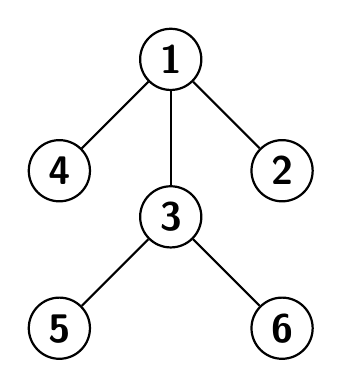
\begin{tikzpicture}[auto, node distance=2cm, every loop/.style={},
	thick,main node/.style={circle,draw,font=\sffamily\Large\bfseries}]
	
	\node[main node] (1) {1};
	\node[main node] (2) [below right of=1] {2};
	\node[main node] (3) [below of=1] {3};
	\node[main node] (4) [below left of=1] {4};
	\node[main node] (5) [below left of=3] {5};
	\node[main node] (6) [below right of=3] {6};
	
	\path[every node/.style={font=\sffamily\small}]
	
	(1) edge node {} (2)
	(1) edge node {} (3)
	(1) edge node {} (4)
	(3) edge node {} (5)
	(3) edge node {} (6);
	
	\end{tikzpicture}
	
	\subparagraph*{3.2}\
	
	First we start by running DFS on the graph. Then when DFS is finished we create a linked list and add the vertices from lowest finishing time to highest finishing time. Now we have a topological sort.\\
	
	After we have the topological sort we can go through the list and find the shortest path.\\
	We do this by going through the list of nodes in the topological graph and counting the length of the path by adding up the predecessors.\\
	
	\begin{lstlisting}[mathescape=true]	
	FindShortestPath(G)
	{
		DFSData = DFS(G) // Run DFS
		// Get the topological sort
		LinkedList l = []
		lowestFinishingTime = min(DFSData.f)
		for v in G
			if DFSData.f[v] == lowestFinishingTime
				l.pushBack(v)
			lowestFinishingTime += 1
		// Find the shortest path
		shortestPath = 0
		for v in l
			if pi[v] == NIL // First node, do nothing
			else
				if pi[pi[v]] == NIL // Predecessor node is origin
					shortestPath = 1 // New tree, so set distance to 1
				else
					shortestPath += 1 // We have travelled an edge
		return shortestPath
	}
	\end{lstlisting}
	
	\subparagraph*{3.3}\
	
	To find a universal sink we can plot a adjacency matrix. When we look at the matrix of a graph with a universal sink we can see that it has an edge from every vertex except itself.
	
	\begin{tabular}{|c|c|c|c|c|c|}
	\hline
	\  & 1 & 2 & 3 & 4 & 5\\
	\hline
	1  & 0 & 1 & 0 & 0 & 0\\
	\hline
	2  & 0 & 0 & 0 & 0 & 0\\
	\hline
	3  & 0 & 1 & 0 & 0 & 0\\
	\hline
	4  & 0 & 1 & 0 & 0 & 0\\
	\hline
	5  & 0 & 1 & 0 & 0 & 0\\
	\hline	
	\end{tabular}\\

Using this knowledge we can define that a vertex which is a universal sink has a link to all vertices except for itself.\\

The algorithm to find a universal sink is as follows:\\ we go through every vertex and go from left to right through the rows, the row needs to have only zeroes.\\ So if we encounter a 1 on a row we go to the next row. If this row has only zeroes to the right we have a probable vertex for our universal sinkhole.\\ To be sure we check that this vertex has no other zeroes in its column.\\

For example, in the above matrix we go start at index 1,1 and see that it is a 0, so we go to the right. We then encounter a 1. In this case index 1 is not an option for the universal sink.\\
After this we go to the next row  and check for zeroes. We then find out that index 2 is an option for the universal sink.\\

After reaching the end of our list of vertices we check our options.\\ This gives us complexity $\mathcal{O}|V|$.

	\subparagraph*{3.4}\
	
To find the mother vertices we first take the Graph in adjacency matrix form. Then we can check if all the values in a row are 1 except for itself. If this is the case then it is a mother vertex.\\

To find out if it is connected to every vertex we need to check the vertices which every successor is connected to and add them to the row of the vertex. When they themselves have successors we need to also add those if we have not added them yet. If we have added them we check the next successor of the vertex.\\

If we can fill the row in this way we have found a mother vertex.\\

Alternative: Run DFS for every vertex, if all other nodes are black and the starting node is still gray, then the starting node must be a mother vertex.
	
	\subparagraph*{3.5}\
	
To get the solution for k=1 we just give the original matrix.\\
And then for k > 1 we need to find the case when there are multiple paths to the destination node given k.\\
To do this we multiply the given matrix by itself k times. So when k = 2 we need to do G $\cdot$ G. And for k > 2 we need to do $G^k$.\\
The result of this multiplication is the answer.

\end{document}